%%%%%%%%%%%%%%%%%%%%%%%%%%%%%%%%%%%%%%%%%%%%%%%%%%%%%%%%%%%%%%%%%%%%%%%%%%%%%%%
% A beamer poster style for the University of Oxford. Atilim Gunes Baydin
% <gunes@robots.ox.ac.uk>, November 2016.
% Based on the I6pd2 style created by Thomas Deselaers an Philippe Dreuw.
%
% Dreuw & Deselaer's Poster
% LaTeX Template
% Version 1.0 (11/04/13)
%
% Created by:
% Philippe Dreuw and Thomas Deselaers
% http://www-i6.informatik.rwth-aachen.de/~dreuw/latexbeamerposter.php
%
% This template has been downloaded from:
% http://www.LaTeXTemplates.com
%
% License:
% CC BY-NC-SA 3.0 (http://creativecommons.org/licenses/by-nc-sa/3.0/)
%
%%%%%%%%%%%%%%%%%%%%%%%%%%%%%%%%%%%%%%%%%%%%%%%%%%%%%%%%%%%%%%%%%%%%%%%%%%%%%%%

% -----------------------------------------------------------------------------
% PACKAGES AND OTHER DOCUMENT CONFIGURATIONS
% -----------------------------------------------------------------------------

\documentclass[final,hyperref={pdfpagelabels=false}]{beamer}

% Use the beamerposter package for laying out the poster with a portrait
% orientation and an a0 paper size
\usepackage{fdsymbol}
\usepackage[orientation=portrait,size=a0,scale=1.3]{beamerposter}
% \usepackage[orientation=landscape,size=a0,scale=1.3]{beamerposter}

\usetheme{NU}

\usepackage[utf8]{inputenc} % allow utf-8 input
\usepackage{blindtext}
\usepackage{amsmath,amsthm,amssymb,latexsym} % For including math equations, theorems, symbols, etc
\usepackage[document]{ragged2e}
\usepackage{times}\usefonttheme{professionalfonts}  % Uncomment to use Times as the main font
\usefonttheme[onlymath]{serif} % Uncomment to use a Serif font within math environments
% \boldmath % Use bold for everything within the math environment
\usepackage{booktabs} % Top and bottom rules for tables
\usepackage{microtype}

\usecaptiontemplate{\small\structure{\insertcaptionname~\insertcaptionnumber: }\insertcaption} % A fix for figure numbering

\newcommand{\shrink}{-15pt}

\def\imagetop#1{\vtop{\null\hbox{#1}}}

\let\oldbibliography\thebibliography
\renewcommand{\thebibliography}[1]{\oldbibliography{#1}
  \setlength{\itemsep}{-10pt}}

% ----------------------------------------------------------------------------
% TITLE SECTION
% ---------------------------------------------------------------------------
\title{\Huge Ad Delivery Algorithms: The Hidden Arbiters of Political Messaging} % Poster title
\author{Muhammad Ali*\textsuperscript{†}, Piotr Sapiezynski*\textsuperscript{†}, Aleksandra Korolova\textsuperscript{‖}, Alan Mislove\textsuperscript{†}, Aaron Rieke\textsuperscript{\S}}
\institute{\textsuperscript{†}Northeastern University; \textsuperscript{‖}University of Southern California; \textsuperscript{\S}Upturn
  %\\\vspace{4mm}
  %\small{\texttt{\{ali.muh, p.sapiezynski, a.mislove\}@northeastern.edu, korolova@usc.edu, aaron@upturn.org}}
  \\\vspace{4mm}\footnotesize{*equal contribution}
  }

% ------------------------------------------------------------------------------
% FOOTER TEXT
% ------------------------------------------------------------------------------
\newcommand{\leftfoot}{* equal contribution} % Left footer text
\newcommand{\rightfoot}{} % Right footer text

% ------------------------------------------------------------------------------
%
% FONT SIZE:
%
% \tiny	sample text
% \scriptsize	sample text
% \footnotesize	sample text
% \small	sample text
% \normalsize	sample text
% \large	sample text
% \Large	sample text
% \LARGE	sample text
% \huge	sample text
% \Huge
% ------------------------------------------------------------------------------
\newcommand\eat[1]{}



% -----------------------------------------------------------------------------

\begin{document}
\addtobeamertemplate{block end}{}{\vspace*{2ex}} % White space under blocks

\begin{frame}[t] % The whole poster is enclosed in one beamer frame

  \begin{columns}[t] % The whole poster consists of three major columns, each of which can be subdivided further with another \begin{columns} block - the [t] argument aligns each column's content to the top

    \begin{column}{.02\textwidth}\end{column} % Empty spacer column

    %%%%%%%%%%%%%%%%%%%%%%%%%%%%%%%%%%%%%%%%%%
    %% Column 1
    %%%%%%%%%%%%%%%%%%%%%%%%%%%%%%%%%%%%%%%%%%

    \begin{column}{.45\textwidth} % 1st column

      \vspace{\shrink}
      \begin{block}{\Large The Problem}
        Can {\it ad platforms} play a role in selectively showing political ads, regardless of how campaigns themselves choose to target? \vspace{1em}
        
        Prior work has shown ad delivery algorithms are capable of biased delivery along race and gender for housing and employment ads \cite{ali-2019-cscw}.
        We ask whether the same effects permeate to political advertising, and affect our democracies adversely. \vspace{1em}

        For the US 2020 elections and Facebook's advertising system, we ask:
        \begin{itemize}
          \item Can the ad delivery algorithm skew delivery by political leaning, even when the advertiser might target broadly?
          \item To what extent does Facebook vary ad pricing based on its hypothesized match between the target audience’s and campaign’s political views?
        \end{itemize}        
      \end{block}

      \begin{block}{\Large Methodology}
        We sign up as political advertisers and run political ads like any campaign would, polling Facebook's ad insights APIs to collect data about performance.
        We run controlled experiments, carefully varying the ad's look, audience size, ad topic and observe how the ad delivery algorithm reacts under identical ad targeting.\vspace{.5em}

        \begin{figure}
          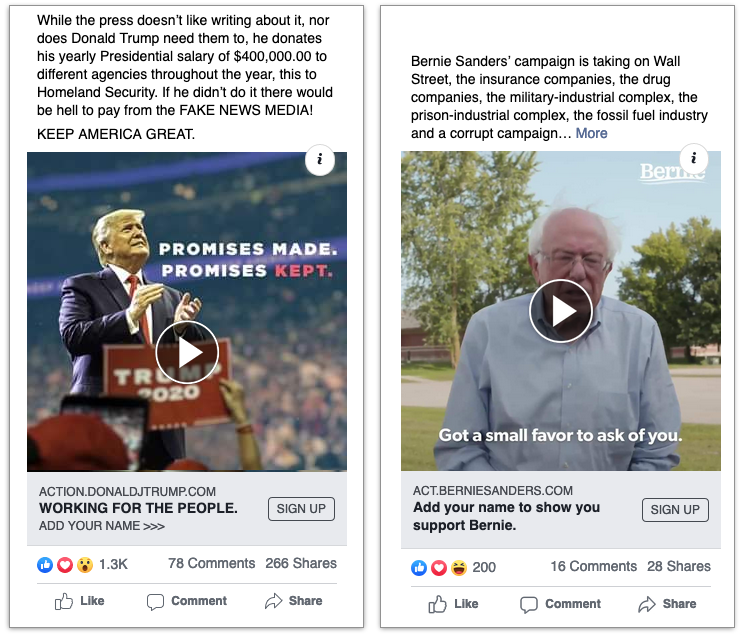
\includegraphics[scale=.9]{figures/ads-issues.png}
          \caption{\hspace{.01em} Ads replicated from Donald Trump's and Bernie Sanders' campaigns.}
          \label{fig:ads}
        \end{figure}
      \end{block}

      \begin{block}{\Large Delivery Skews and Price Discrimination}
        We find that, despite identical targeting, the same Trump or Sanders ad reaches more people when targeted to audiences that might already agree with the message.\vspace{.5em}

        \begin{figure}
          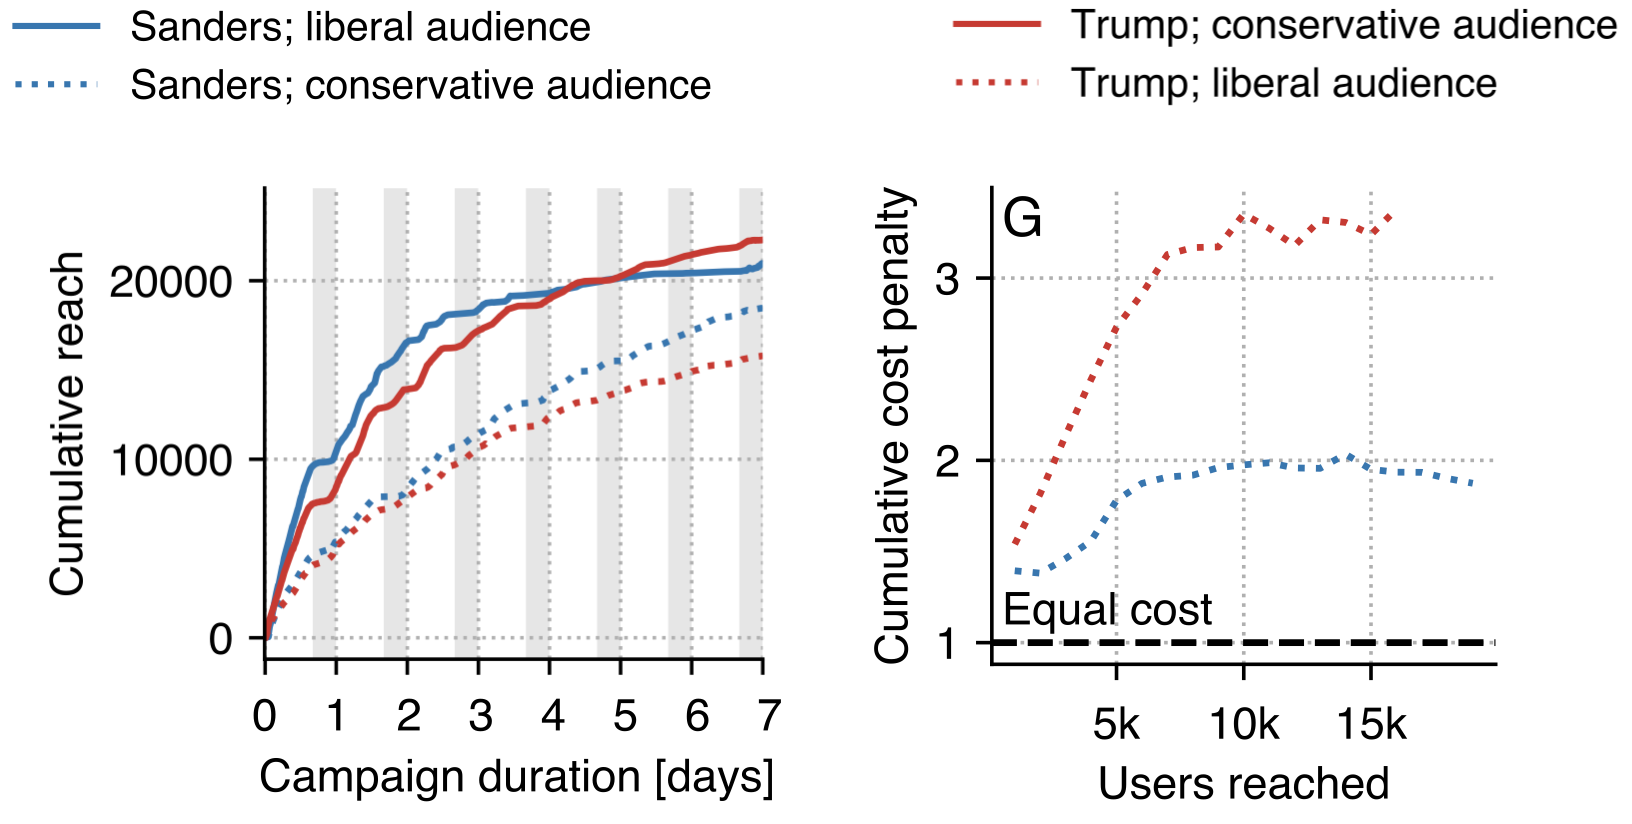
\includegraphics[scale=1.25]{figures/result-1.png}
          \caption{\hspace{.01em} Reach differences for conservative and liberal audiences (left), and price differences (right), for both Trump and Sanders ads.}
        \end{figure}

        Our experiments also show the large premium a political campaign might have to pay to reach users that (according to Facebook) do not have a matching political leaning.\vspace{1em}

        Our ads here are taken from the original campaigns (Figure~\ref{fig:ads}), optimized to reach as many people as possible, run at the same time, and with the same budget.
      \end{block}
    \end{column} % End of the 1st column

    %%%%%%%%%%%%%%%%%%%%%%%%%%%%%%%%%%%%%%%%%%
    %% Column 2
    %%%%%%%%%%%%%%%%%%%%%%%%%%%%%%%%%%%%%%%%%%

    \begin{column}{.02\textwidth}\end{column} % Empty spacer column

    \begin{column}{.45\textwidth} % 2nd column
      \vspace{\shrink}
      \begin{block}{\Large The Effects of Ad Content}
        We find that delivery skews and price differences persist even when running ads that look {\it exactly} the same to users. Having identical ad copies allows us to control for any user interactions that might impact delivery.\vspace{1em}

        We set up our web server so that any traffic from actual users is redirected to \texttt{https://fec.gov}, while Facebook-internal IPs are either served a Sanders or a Trump page.\vspace{.5em}

        \begin{figure}
          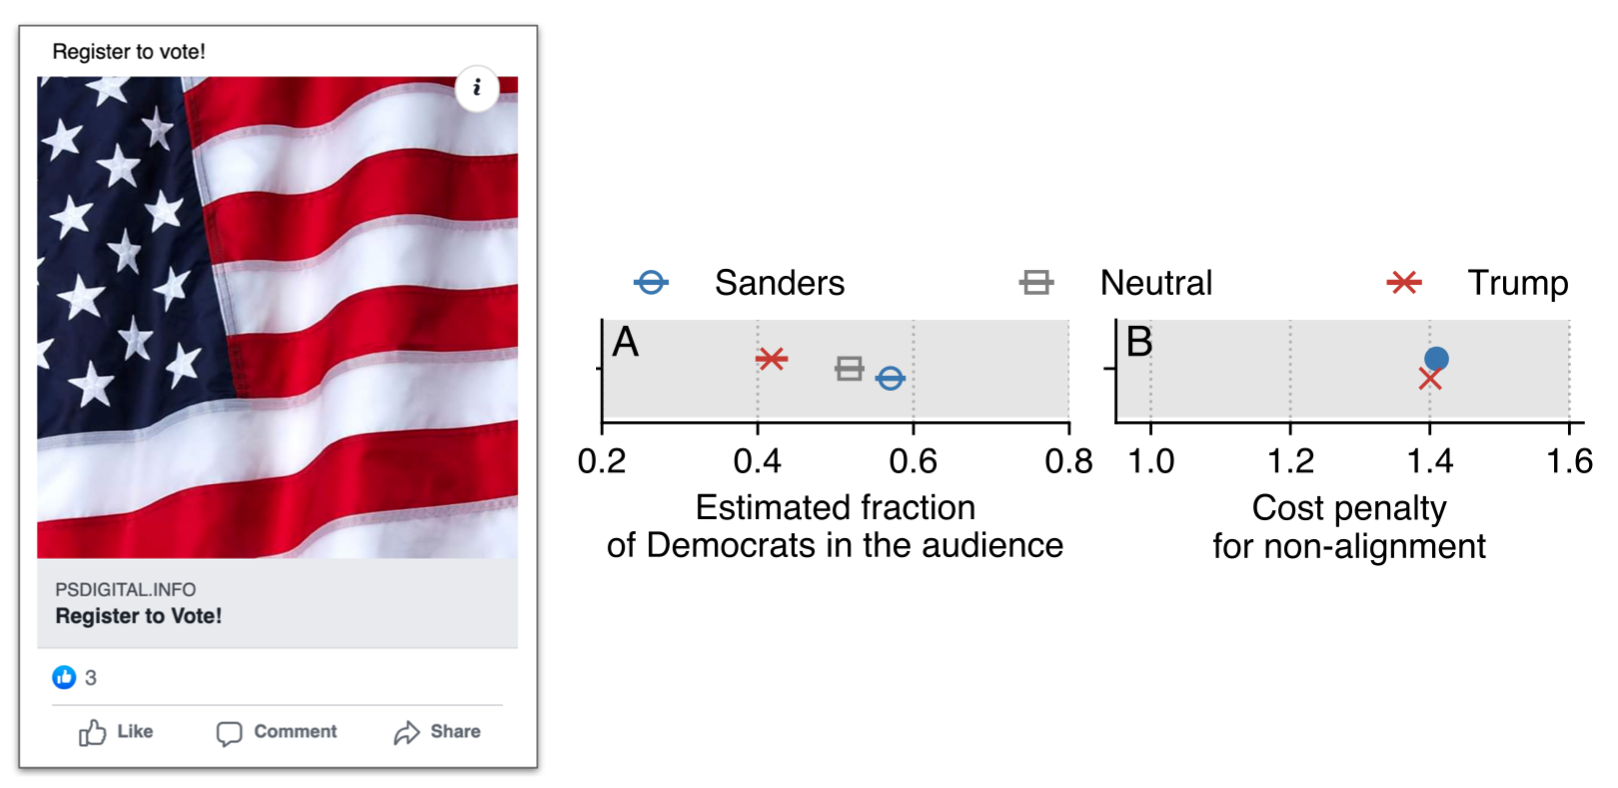
\includegraphics[scale=1.25]{figures/result-2.png}
          \caption{\hspace{.01em} Results on ad that looks identical to users but presents different campaigns to Facebook.}
        \end{figure}

        This shows that the platform's classification of content plays a significant role in the ad's eventual performance, and can lead to sometimes unexpected delivery skews and price differences.
      \end{block}

      \begin{block}{\Large Consequences}
        Facebook limits political advertisers’ ability to reach audiences that do not share those advertisers’ political views in ways that are significantly different from traditional broadcast media.\vspace{1em}

      \begin{itemize}
        \item The existence and extent of this skew may not be apparent to advertisers and varies based on their ad’s message as well as the destination link used by the campaign.\vspace{1em}
        \item Limiting advertisers' targeting options (e.g. disallowing microtargeting), without a discussion of the role of ad delivery, is only half the picture\vspace{1em}
        \item There is precedent for regulating the power of broadcasting platforms, such as ``Equal-Time Rule'' for broadcast licensees~\cite{EqualTimeRule} --- it is logical to ask these questions of online ad platforms to hold them accountable.\vspace{1em}
      \end{itemize}

      Researchers, regulators, and political campaigns today lack access to algorithms and data required for a more thorough study of ad delivery implications.
      Blackbox algorithm auditing is one of the first steps towards understanding and mitigating the adverse effects of these systems.
      \end{block}

      \begin{block}{\Large References}
        \nocite{*} % Insert publications even if they are not cited in the poster
        \linespread{0.928}\selectfont
        \footnotesize{\bibliographystyle{unsrt}
          \bibliography{nu_poster}}
      \end{block}

    \end{column} % End of the 2nd column


    \begin{column}{.02\textwidth}\end{column} % Empty spacer column

  \end{columns} % End of all the columns in the poster
\end{frame} % End of the enclosing frame
\end{document}
